\section{COStream数据流编程语言及其在深度学习中的应用(于俊清)}
\subsection{引言}
随着半导体技术的发展,未来的高性能处理器将会在单块芯片上集成数十个甚至数百个处理核心。近些年,多/众核架构已经被普遍认为是开发并行性的有效平台,一方面它为各类应用提供了强大的并行计算能力,特别是在数字媒体处理和科学计算等计算密集型的应用领域;另一方面它也将如何充分的挖掘程序的并行性以及如何充分的利用资源等问题暴露给了编程人员。传统的编程模型,如C、C++和Fortran,主要对应的都是单指令流和集中存储管理模式,无法很好的适合这种特殊的并行体系结构。当前比较流行的编程模型,如OpenMP和MPI,要求程序员必须熟悉并行系统的底层结构,编程人员设计并行程序时需要根据系统底层结构进行精心的任务划分、数据通信以及同步设计。导致了程序性能受制于编程人员并行算法的设计和对并行系统的理解,极大地增加了编程人员,尤其是各个应用领域编程人员的编程负担。
针对上述问题,数据流编程模型作为新的高效的并行编程模型被提出来,编译器可以根据多核处理器体系结构的特点有效的将任务进行划分并映射到各个处理核上,生成适合于当前体系结构的可执行程序,大大简化编程难度,提高程序执行的效率。

基于多核与分布式系统结构以及数据流编程模型的特点,华中科技大学的智能媒体计算与网络安全实验室设计并实现了一种面向数据流编程的编译系统 -- COStream。语言的名称由3个关键字:Composite、Operator和Stream组合而来。COStream程序采用有向图来描述应用的处理过程,图中节点表示计算,边表示数据依赖,边的方向表示数据流动方向。下文从几个小节进行介绍: 5.2.2编程语言设计;5.2.3编译器框架; 5.2.4~5.2.5面向不同平台的编译优化; 5.2.6深度学习程序开发实例



\subsection{COStream 数据流编程语言}
COStream是在C语言文法基础上加入了表征数据流图结构文法而形成的数据流编程语言,它实现了对数据流图最基本的抽象,方便数据流程序的编写。语言的名称由3个关键字:Composite、Operator和Stream组合而来。

\subsubsection{与 C 语言的联系与区别}
(1)COStream 保留了 C 语言的全局变量声明, 在文件头部声明了全局变量名后, 可以在后续的函数,Composite 和 Operator 中使用。下面给出了一些示例代码:
\begin{algorithm}\label{algo:standard}
int i = 0; double j = 0.0; //支持整数和浮点数\\
int i = 1, j = 2, k = 3; //支持一条语句中声明多个变量\\
int i = 1e10, j = 0x16; //初始值支持科学记数法和16进制\\
int a[3] = { 1,2,3 };   //支持数组声明和赋初值
\end{algorithm}

(2)COStream 支持全局函数声明,但由于其是数据流编程语言,而非面向对象编程语言,不能通过 this 关键字来访问执行上下文, 因此全局函数多用来做一些数据计算的复用,下面给出一些示例:

\begin{algorithm}\label{algo:standard}
int sum(int a, int b)\{\\
\hspace*{1 pc} return a+b; // 最基础的加法运算\\
\}\\
double expr(double base, double x)\{\\
\hspace*{1 pc} return base**x; // 支持使用两个星号**来表示 base 的 x 次方\\
\}
\end{algorithm}
(3)COStream 支持的基础运算类型有: 
\begin{itemize}
    \item 双目运算符: + 加, - 减, * 乘, / 除, \% 取余, ** 乘方
    \item 位运算符: \& 按位与, | 按位或, \^{} 异或, << 左移, >> 右移
    \item 逻辑运算符: < > <= >= == != \&\& || !
    \item 单目运算符: + 正号, - 负号, ++ 自增, -- 自减
    \item 三目运算符: ? :
    \item 成员运算符: . 例如 S.a
\end{itemize}

但与 C 语言不同的是, COStream 抛弃了 C 语言中函数必须先声明后调用的限制, 而参考其它语言的文法, 规定函数的调用可以放在声明前, 实现方式为通过编译器在文法解析时的预处理, 优先将全局变量和函数声明信息存入符号表, 使得解析函数调用时可以直接从符号表中提取相关信息, 而非依赖上下文环境。

\subsubsection{Operator}

同步数据流图中最基本的组成单元和计算单元actor在COStream中由operator文法结构表示,operator在SDF中被抽象成一个结点,专门用来处理stream中的数据。operator定义了actor输入流、输出流和具体的处理过程。operator由头部定义和体定义组成,其中operator头部定义了该operator处理的输入、输出流以及operator名称,COStream暂时不支持匿名operator的定义。COStream中一个operator可以有多个输入流和多个输出流。Operator体包括declare(静态变量声明)、init(静态变量初始化)、work和window四个部分。其中,work函数是operator内最细粒度的运算,是operator的核心结构,是数据流程序迭代执行过程中每次执行计算的单元。对operator输入和输出缓冲区的访问操作也是在work中进行的。operator内部变量的声明部分(declare)主要是为了定义该operator的work在执行时是需要的一些静态变量,类似于C语言中static关键字修饰的变量,对于无状态的operator来说,这部分可以为空。init定义了operator开始执行时需要进行的初始化工作。window规定输入、输出数据流缓冲区的窗口类型并决定operator对输入、输出流中数据访问的窗口大小。下面给出一个示例, 该示例描述了一个产生1,2,3,4,5,6...的自然数序列的数据流。

\begin{algorithm}\caption{产生自然数序列的数据流示例}\label{algo:operator-example}
  stream<int x>S;\\
  S = Source()\{\\
  \hspace*{1 pc} int i;\\
  \hspace*{1 pc} init \{i = 1;\}\\
  \hspace*{1 pc} work \{\\
  \hspace*{2 pc} S[0].x = i;\\
  \hspace*{2 pc} i++;\\
  \hspace*{1 pc} \}\\
  \hspace*{1 pc} window\{\\
  \hspace*{2 pc} S tumbling(1);\\
  \hspace*{1 pc} \}\\
  \};
\end{algorithm}

该示例的第1行描述了一个由整数int组成的数据流 S, 可以使用S[0]来访问数据流 S 的窗口中第一个位置, 而 S[0].x 表示该位置的成员 x (其类型为 int)。 接着,在示例的3~4行,Operator Source 声明了一个静态变量 i 并赋初值为1,接下来的执行流程为:执行一次 work 内部的语句->翻转窗口window->执行一次work内部语句->翻转窗口 window->…->执行一次work内部语句->翻转窗口window, 可以看出, 每次执行 work 都会使得窗口第一个位置的 x 赋值为自然数序列变量 i 的最新值 同时 i 自增,然后通过 window 中的窗口翻转将该数据传给后续的 Operator。

下面详细讨论COStream中的窗口机制。
\begin{figure}[htbp]
	\centering
	% Requires \usepackage{graphicx}
	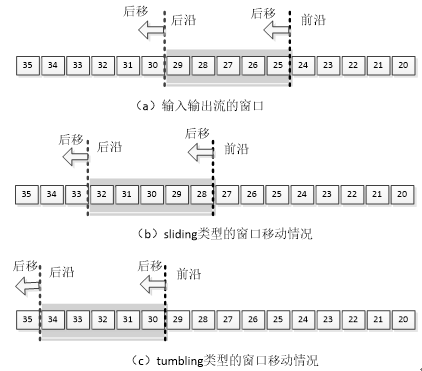
\includegraphics[width=5in]{Img/Chap_Application/Yu/operator.png}\\
	\caption{operator的窗口机制}\label{fig:operator}
\end{figure}
COStream对流中的数据访问采用窗口机制,窗口用前沿和后沿界定,前沿和后沿的距离就是当前operator执行时可操作的输入、输出缓冲区的大小,它由window中的参数确定。COStream中窗口类型有两种:sliding和tumbling。sliding代表滑动窗口类型,这种窗口有peek,pop和push操作,一般用于输入流;而tumbling则代表翻转窗口类型,只有push和pop操作,该种类型窗口既可以用于输出流也可以用于输入流。对于输入流主要的操作有pop和peek。pop操作删除输入流中最先到的token,并返回该token。peek(i)返回输入流中距离输入流窗口前沿的第i个token。对于输出流主要操作是push,push操作是将计算得到的token输出到输出流,对缓冲区的使用是从前沿到后沿的。operator一次执行完成后同时移动窗口的前沿和后沿。图\ref{fig:operator}(a)图描述COStream中的输入输出流的窗口示意图,图\ref{fig:operator}(b)和(c)分别表示如果(a)对应的窗口分别是sliding(5,3)和tumbling(5)时,一次operator执行完成后窗口的移动情况。


\subsubsection{Composite}
在面向过程编程的 C 语言中, 程序入口为 main 函数, 在函数中使用多种控制语句来编写程序。与之不同,在面向数据流编程的 COStream 语言,程序入口为 Composite Main,在其内部通过将不同 Operator 用Stream 变量进行连接来构造数据流图。

COStream定义的用于连接不同节点构造数据流图的Composite结构属于高层次(相对于operator)的复合结构,代表一个由一个或若干个operator组成的可重用的数据流图结构,它是对SDF图中可复用的子图的抽象。它既可以完整的表示一个数据流程序的数据流图结构,也可以作为子数据流图结构被调用。下面是一个略去细节信息的抽象 composite 例子,它表示输入的数据流 S 依次经过了3个 operator 的处理后,计算得到了输出流T。

\begin{algorithm}\label{algo:operator}
Composite Main(input S, output T)\{\\
 \hspace*{1 pc} S0 = first(S);\\
 \hspace*{1 pc} S1 = second(S0);\\
 \hspace*{1 pc} T  = third(S1);\\
\}
\end{algorithm}

composite主要由composite头部和composite体组成。composite头部表明该composite的输入输出边参数、composite参数以及composite的名称,COStream不支持匿名composite。composite的输入输出边参数是用来确定在生成SDF图时该composite结构所形成的子图与SDF图中其他节点的连接关系。composite参数主要是指composite结构在实际被调用时需要从调用处传入的参数,可以根据参数的情况决定composite最终子图的结构,另外该参数也可以在composite内部被使用。composite体主要有如下2部分组成:一部分是composite内部需要使用的变量的定义和一些相关的操作语句;另一部分是composite内部的子图结构,它由一个或若干operator组成,每个operator根据输入流、输出流的依赖关系连接成图,是composite的核心结构。Composite结构在编译阶段被扩展,经过编译数据流程序的数据流图子结构将被扩展成完整的数据流图。

\subsubsection{多输入多输出流的连接方式}

composite可以同时有多个输入多个输出边。下面的数据流程序例子反映了上述语言特点。

\begin{algorithm}\label{algo:operator}
composite M (output K,L,input G,H) \{		//1\\
 \hspace*{1 pc} stream<int x> I=O(G)\{\}			//2\\
 \hspace*{1 pc} stream<int x> J=P(H)\{\}			//3\\
 \hspace*{1 pc} stream<int x> K=Q(I;J)\{\}			//4\\
 \hspace*{1 pc} stream<int x>L=R(J)\{\}			//5\\
\}									//6\\
composite Main\{						//7\\
 \hspace*{1 pc} …\\
 \hspace*{1 pc} (stream<int x>C,stream<int x> D) = M(A,B)\{\}	//8\\
 \hspace*{1 pc} (stream<int x>E,stream<int x> F) = M(A,B)\{\}	//9\\
 \hspace*{1 pc} …\\
\}
\end{algorithm}

\begin{figure}[htbp]
	\centering
	% Requires \usepackage{graphicx}
	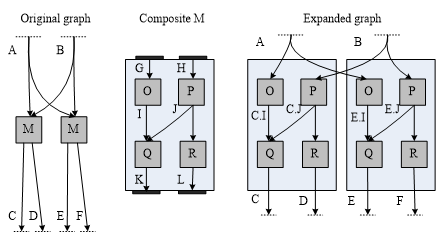
\includegraphics[width=1.0\textwidth]{Img/Chap_Application/Yu/multi.png}\\
	\caption{多输入多输出流连接方式}\label{fig:multi}
\end{figure}

图\ref{fig:multi}描述了行1至行9的程序片段所反映的数据流图调用、扩展过程:由Original graph扩展为Expanded graph。Original graph包含了2个composite结构M,第一个M将输入流A和B计算后得到输出流C和D,第二个M将输入流A和B计算后得到输出流E和F。行1定义了M的输入流为G和H,输出流为K和L。行8表示当M在Main中第一次被调用时,输入流和输出流发生实例化:G=A,H=B,K=G以及L=D。在Expand graph中M因为被调用2次而实例化成2份,所以M中的中间流I和J也被实例化为2份:C.I,C.J和E.I,E.J。这些子流图因被调用而实例化展开的过程在编译器编译时完成,经过编译后,数据流程序的流图结构将被扩展成完整的数据流图。

\subsubsection{pipeline 连接方式}

\begin{figure}[htbp]
	\centering
	% Requires \usepackage{graphicx}
	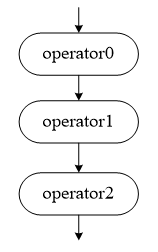
\includegraphics[width=0.25\textwidth]{Img/Chap_Application/Yu/pipeline.png}\\
	\caption{pipeline连接方式}\label{fig:pipeline}
\end{figure}

有时候我们会想要编写这样一种数据流结构: 每个 operator 的输入恰好是上一个 operator 的输出,即数据流在全局或局部保持单向传递,有时 operator 还可以复用。例如对应图\ref{fig:pipeline}中有3个 operator 的示例:

\begin{algorithm}\label{algo:costream}
Composite Main(input<int x> S0)\{\\
 \hspace*{1 pc} stream<int x>S1,S2,S3;\\
 \hspace*{1 pc} S1 = operator0(S0);\\
 \hspace*{1 pc} S2 = operator1(S1);\\
 \hspace*{1 pc} S3 = operator2(S2);\\
\}
\end{algorithm}

在这种情况下, 我们最关心的是输入流变量 S0和输出流变量 S3,而数据流变量S1,S2是多余的信息,实际上我们并不关心中间变量。在其它函数式编程语言中,我们可以使用 compose(组合)这个操作符来描述这种结构:

\begin{algorithm}\label{algo:costream}
operator3 = compose(operator0,operator1,operator2)\\
S3 = operator3(S0)
\end{algorithm}

等价于

\begin{algorithm}\label{algo:costream}
S3 = operator2(operator1(operator0(S0)))
\end{algorithm}

那么在COStream 数据流编程语言中, 有没有这种”串联”形式的组合结构呢?答案是有的, 这就是 pipeline 结构, 下面给出对应示例:

\begin{algorithm}\label{algo:costream}
Composite Main(input<int x> S0)\{\\
 \hspace*{1 pc} S3 = pipeline(S0)\{\\
 \hspace*{2 pc} add operator0();\\
 \hspace*{2 pc} add operator1();\\
 \hspace*{2 pc} add operator2();\\
 \hspace*{1 pc} \}\\
\}
\end{algorithm}

pipeline结构是由一串连续的composite调用组成,它们在pipeline结构中出现的先后顺序决定了它们在数据流图中的依赖关系。pipeline是单输入流单输出流,COStream规定能够在pipeline中被调用的composite也必须是单输入流单输出流。

\begin{algorithm}
  \caption{代码片段 A 和使用了 for/if 的代码片段 B 等价}
  \label{algo: pipeline}
  {\bf 代码片段 A}\\
  Composite Main(input<int x> S0)\{\\
    \hspace*{1 pc} S3 = pipeline(S0)\{\\
    \hspace*{2 pc} add operator0();\\
    \hspace*{2 pc} add operator1();\\
    \hspace*{2 pc} add operator0();\\
    \hspace*{2 pc} add operator1();\\
    \hspace*{2 pc} add operator0();\\
    \hspace*{2 pc} add operator1();\\
    \hspace*{1 pc} \}\\
  \}\\
  {\bf 代码片段 B}\\
  Composite Main(input<int x> S0)\{\\
    \hspace*{1 pc} S3 = pipeline(S0)\{\\
    \hspace*{2 pc} for(int i=0;i<3;i++)\{\\
    \hspace*{3 pc} if(i\%2==0)\{\\
    \hspace*{4 pc} add operator0();\\
    \hspace*{3 pc} \}\\
    \hspace*{3 pc} else\{\\
    \hspace*{4 pc} add operator1();\\
    \hspace*{3 pc} \}\\
    \hspace*{2 pc} \}\\
    \hspace*{1 pc} \}\\
  \}
\end{algorithm}

COStream引入add操作将operator和composite调用添加到pipeline中。 此外, pipeline 的结构体中支持使用 if 、for、while 语句等来控制 operator 的组合, 如算法\ref{algo: pipeline}所示,我们可以把代码片段 A 改写为代码片段 B,二者是等价的。





\subsubsection{splitjoin 连接方式}

\begin{figure}[htbp]
  \centering
  % Requires \usepackage{graphicx}
  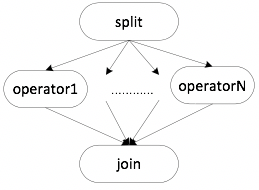
\includegraphics[width=0.5\textwidth]{Img/Chap_Application/Yu/splitjoin.png}\\
  \caption{splitjoin连接方式}\label{fig:splitjoin}
\end{figure}

除了 pipeline结构, 还有一种 splitjoin 结构用来描述数据流的分解与合并(图\ref{fig:splitjoin})。splitjoin结构由splitter、joiner以及一些composite调用组成,当一个流作为splitjoin结构的输入流时它被splitter分割,splitter根据splitjoin中composite调用情况产生一批满足相应条件的输出流作为不同的composite调用的输入流,这些composite调用的输出流作为joiner的输入流,joiner同样根据composite调用情况来合并各个输入流,将合并后产生的新的流作为joiner结点的输出,也是splitjoin结构的输出流。在splitjoin中splitter主要有两种方式:

\begin{itemize}	
  \begin{figure}[htbp]
    \centering
    % Requires \usepackage{graphicx}
    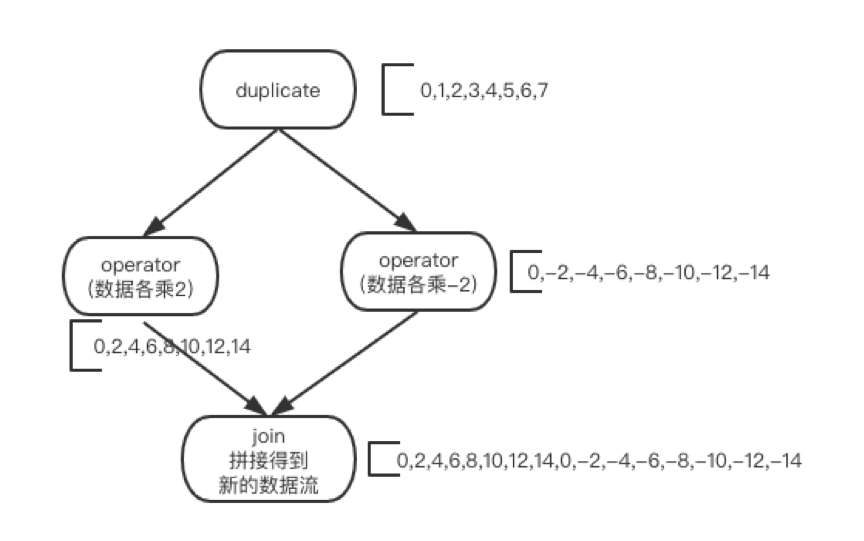
\includegraphics[width=0.8\textwidth]{Img/Chap_Application/Yu/duplicate.png}\\
    \caption{splitjoin-duplicate示意图}\label{fig:duplicate}
  \end{figure}

  \item {\bf duplicate方式}:该方式下所有的composite调用将会有完全相同的输入流。如图\ref{fig:duplicate}所示:

  \begin{figure}[htbp]
    \centering
    % Requires \usepackage{graphicx}
    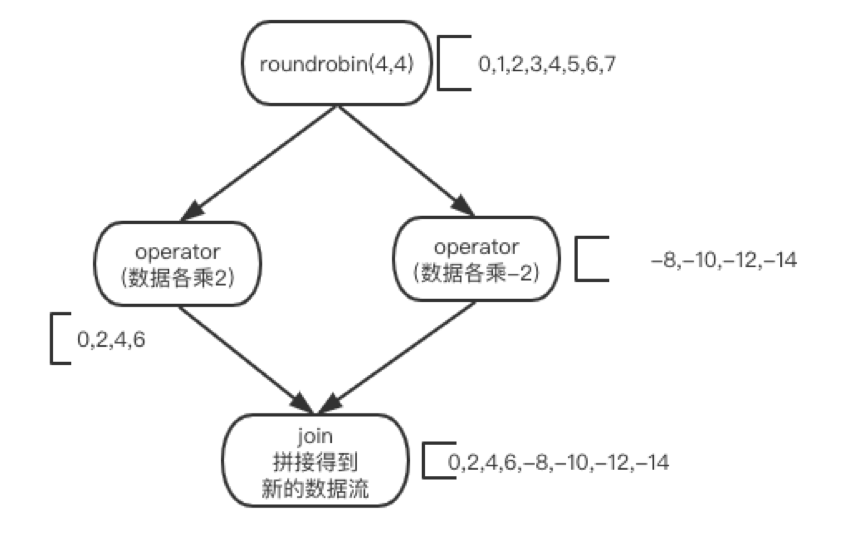
\includegraphics[width=0.8\textwidth]{Img/Chap_Application/Yu/roundrobin.png}\\
    \caption{splitjoin-roundrobin示意图}\label{fig:roundrobin}
  \end{figure}

  \item {\bf roundrobin(w1,…,wn)方式}:如图\ref{fig:roundrobin}所示,该方式下splitter将其输入流中的前w1个数据发送给第一个composite调用,接下来的w2个数据发送给第二个composite调用,以此类推,将最后的wn个数据发送给最后一个composite调用。对于joiner只有一种roundrobin方式。与pipeline结构类似,在splitjoin中调用的composite要求也是单输入流和单输出流的。
\end{itemize}

在COStream中splitter和joiner分别用关键字split和join表示,且可以和 pipeline 结构互相嵌套使用,下面是一个示例:

\begin{figure}[htbp]
  \centering
  % Requires \usepackage{graphicx}
  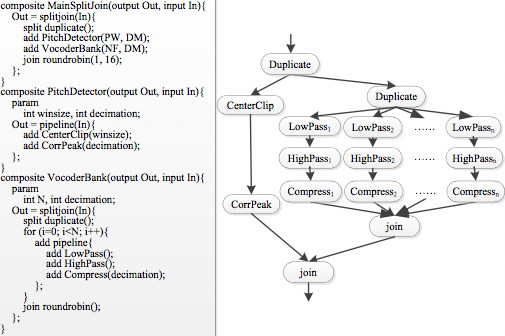
\includegraphics[width=1.0\textwidth]{Img/Chap_Application/Yu/vocodebank.png}\\
  \caption{vocodebank程序例子}\label{fig:vocodebank}
\end{figure}

图\ref{fig:vocodebank}的例子能够说明splitjoin和pipeline的层次性特点和使用特性。在图中左边部分是COStream的源码片段,右边是对应的数据流图。在本例中可以看到添加了层次性的结构有助于增加数据流程序编程的灵活性和可扩展性。另外,在splitjoin和pipeline中流能够被参数化,在本例composite VocodeBank中关于内置的pipeline调用次数可以有参数N来确定,通过N控制splitjoin结构的宽度,同样在pipeline中可以通过参数来控制pipeline的深度。

\subsubsection{内置 composite}

为了便于对文件操作,COStream对文件的I/O提供了内置composite支持,通过调用内置的文件I/O composite COStream可以完成对文件读写操作。FileReader和FileWriter是COStream为I/O提供的内置的composite接口。FileReader用于将文件中的数据读到流中,FileWriter是将流中的数据写到文件中。具体用法如下:

\begin{algorithm}\label{algo:costream}
stream<double x> A,B;			//1\\
A = FileReader(“data.bin”);		//2\\
FileWriter(B)(“result.txt”);
\end{algorithm}

行1表示将data.bin文件中的数据读入到数据流A中,行3表示将处理后输出的流B中的数据保存至文件result.txt。

此外,仍然存在许多常用能性 Composite有待于内置在COStream编程语言中, 实验室的全体师生会积极进行版本迭代,进一步改进和优化COStream的编程语言结构设计。 

\subsection{COStream 编译器框架简介}

前文介绍了 COStream 数据流编程语言, 由此我们可以根据有限的文法来组合出想要的数据流程序。但人类编写的数据流程序对于计算机来说只是一串文本字符串,必须经过特定编译器的编译才能转化为对应的可执行程序。下面介绍由华中科技大学的智能媒体计算与网络安全实验室设计并实现的COStream数据流编程的编译系统。

\begin{figure}[htbp]
  \centering
  % Requires \usepackage{graphicx}
  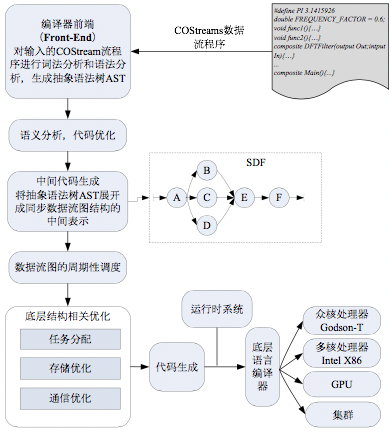
\includegraphics[width=0.8\textwidth]{Img/Chap_Application/Yu/compiler.png}\\
  \caption{COStream 编译器框架示意图}\label{fig:compiler}
\end{figure}

图\ref{fig:compiler}描述了COStream编译系统总体框架。COStream编译器的源语言为COStream数据流程序设计语言,目标语言根据目标结构不同生成不同底层语言,如C、C++(在x86平台上执行)和openCL(在 GPU 上执行)以及 Javascript(在跨平台的浏览器中执行)等,编译器通过调用底层语言编译器生成对应目标平台的可执行文件。下面详细介绍COStream编译系统的组成部分。

\begin{itemize}	
  \item {\bf 编译器前端}:编译器前端主要对COStream源程序进行分析,建立抽象语法树。对源程序的分析主要包括词法分析和语法性分析。在词法分析中,词法分析器从左到右地读构成源程序的字符流,把字符流分组为多个记号,记号是具有整体含义的字符序列。词法分析通常作为编译器的第一个阶段,产生记号序列,提交给语法分析使用。这里将词法分析作为语法分析的子程序来实现。当词法分析器收到语法分析器发出“取下一个记号”的命令时,词法分析器读入字符,识别出一个记号。COStream采用自底向上的语法分析过程。在语法分析中,将字符串或者记号划分为具有一定层次的多个嵌套组,每个嵌套组具有一个完整的含义。程序的层次性结构是通过递归规则来表达,在编译器中,语法分析器接受词法分析器提供的记号串,检查它们是否符合COStream的文法规则。如果文法匹配则通过规则建立语法树结点结构。源程序通过词语法分析最终将建立为一种由顶层语法树节点表示的层次性抽象语法树结构。COStream采用Lex和Yacc词语法生成器生成词语法分析器。

  \item {\bf 语义分析和代码优化}: 编译器对经过词语法分析形成的抽象语法树进行语义分析。语义分析是对COStream数据流程序进行类型检查以及为代码生成阶段收集类型信息。语义检查负责检验每个操作符的操作数是否满足源语言的说明。在该阶段除语义检查外还对源程序代码做机器无关优化。优化是在保持源程序语义的基础上减少代码占用空间,删除不必要的操作,降低程序运行时开销。为了提升程序的性能COStream实现了常见的机器无关优化,如常量传播和冗余代码删除等。该阶段得到最佳抽象语法树。
  \item {\bf 中间代码生成}: COStream编译器以同步数据流图作为中间表示,在该阶段分析编译器前端得到的抽象语法树,得到数据流程序中的composite调用关系和stream依赖关系,利用这两种关系将抽象语法树进行深层次的展开,得到一个只有operator通过stream相连的完整的数据流图的抽象语法树结构,利用此时的抽象语法树生成SDF图,该SDF图是编译器后续操作的基础。另外,在该阶段还需要对SDF图中的各个节点的工作量进行估计,确定SDF图中各个actor的负载情况。
  \item {\bf 数据流图的周期性调度}: 编译器根据中间表示的数据流图结构采用单出现调度策略 (Single Appearance Schedule,SAS) 得到静态平衡数据流图。编译器根据程序中各个operator的peek、pop和push率决定初态和稳态调度阶段的各个actor的执行次数,为后续的优化和代码生成提供依据。
  \item {\bf 底层结构相关优化}: 编译器根据不同底层系统结构特性,对COStream程序进行与底层结构相关的优化,主要从计算任务分配、存储优化和通信优化等方面对程序进行优化,在开发并行性的同时减小相应的开销,使数据流程序在执行时能够充分利用底层系统的资源,提高程序的执行效率。COStream主要针对X86、GPU和多核集群等目标系统做编译优化。在第5.2.4节中具体介绍面向X86共享多核架构下的相关优化。
  \item {\bf 代码生成}: 根据底层结构相关优化的结果和后端的体系结构以及目标代码的特性,设计最终目标代码的生成框架,生成高效的可并行代码。
  \item {\bf 运行时系统}: 运行时系统是采用目标语言编写的静态链接库,包括支持目标代码运行所需要通信库和函数库,为代码生成提供辅助支持。
  \item {\bf 底层编译器}: 编译器将生成的目标底层代码交由底层语言编译器编译生成指定目标平台的可执行文件,完成整个编译过程。
  
\end{itemize}

\subsection{面向 X86 多核集群的 COStream 编译优化}

随着多核处理器平台日趋复杂,数据流程序的并行编译优化工作变得更加困难,其问题主要包括多处理器核的并行调度和对主存的访问延迟。针对数据流程序根据共享存储多核架构的结构特点,构造出高吞吐量低延迟的软件流水线调度,主要分为任务划分、阶段赋值、流水线执行三个步骤。

\subsubsection{任务划分}

任务划分是在避免浪费处理器核的计算能力以及确保各处理器核间的任务负载均衡的基础上,使用合适的划分算法将数据流任务划分到合适的核上。任务划分的目的是根据数据流图(SDF图)中计算节点的负载和计算节点间的依赖关系构造高吞吐量低延迟的软件流水线调度,以最大化底层系统资源利用率。数据流程序要想充分利用系统资源就必须充分合理地利用其自身的数据并行性、任务并 行性和流水线并行性。在软件流水线调度中,流水线的启动间隔(Initiation Interval,II)是指相邻两次循环迭代进入流水线的时间间隔,II越小意味着吞吐率越大。任务划分的目的就是要最小化II。在软件流水中II是由流水线中各资源的处理时间决定,在X86中,资源主要是处理器核,那么影响程序最终执行性能的主要因素就是划分的负载均衡情况。

在进行任务划分前,需要对SDF进行预处理,包括扩大调度和融合相邻计算节点。扩大调度指的是以相同的扩大因子,成倍扩大每个计算单元稳态调度阶段的执行次数,这样可以减少同步开销对程序性能的影响。相邻计算节点的融合是指将两个独立且在数据流图中相邻的计算节点融合为一个计算单元。相邻

计算单元融合操作保证了两个计算单元不会被分配到不同的处理器核上调度,这能够减少通信开销对程序的影响; 但是过度的融合操作会减少数据流图的计算单元,可能导致任务划分阶段负载的不均衡。相邻计算单元融合算法的关键在于如何判断是否某对相邻计算单元进行融合。首先,被融合的计算单元必须是单输入单输出的,这是由于过多的通信边将导致复制分裂后计算单元间过多的通信开销;其次,因为存在状态计算单元不能进行数据并行调度,所以不对相应状态计算单元进行融合操作。对于满足上述两个条件的相邻节点,根据两者通信量之和以及融合后的计算量,当通信计算比大于某个阈值时,将其合并为一个计算单元。

在对SDF图进行预处理优化后,在此基础上采用划分算法来进行任务划分。COStream 任务划分采取以负载均衡为目标同时最小化同步通信开销的分配策略。负载均衡的目的是为了保证流水线在满状态时各个核上的有效计算时间是相等的,核间因相互等待而产生的空闲时间将会小,II就会小,处理核利用率就高,系统的吞吐量就大。同时,因为SDF中计算节点之间有数据依赖,为了保证数据访问的局部性最小化同步通信延迟,在任务划分时应该尽可能地将有依赖关系的计算节点分配在一个核上以最大程度地减少核间通信边的数量。文献比较了常见的任务划分和分配策略,常见的分配策略主要包括有循环分发分配策略、亲和性分配策略和贪心分配策略等。综合COStream程序运行时存在的问题及常见任务分配策略,COStream选择以负载均衡为目标同时最小化通信开销的 K路图划分算法(MultilevelK-way Partitioning,MKP)。COStream采用Metis提供的接口实现MKP算法为SDF图作任务分配。由于MKP作为通用的图划分算法,没有充分结合数据流程序自身存在的各种并行性其结果并不能很好地满足程序运行的要求,COStream在MKP划分结果的基础上根据数据流程序的特点进行了进一步优化,提出复制分裂算法,图9描述了复制分裂算法的基本流程。复制分裂算法根据 MKP 划分结果的负载平衡情况,利用了SDF图中无状态的计算节点存在的数据并行性,对无状态的计算节点做分裂,增大任务并行性,将分裂产生的不同副本分配到不同的划分子集中,降低计算节点粒度,使不同划分的负载达到平衡。经过实验分析看到,COStream在X86环境下平衡因子设为1.5时能够得到较理想的结果,其中平衡因子指的是划分中负载最大的与最小的比值。

\subsubsection{阶段赋值}

\begin{algorithm}
  \caption{阶段赋值算法}
  \label{algo:stage}
  输入:SDF图G(V,E),图G计算单元到核的映射actorProcMap\\
  输出:图G计算单元到阶段号的映射actorStageMap\\
  1.	topologicalOrder = topologicalTrav();\\
  2.	for all actor v in topologicalOrder do\\
  3.	  \hspace*{1 pc} int maxStage = 0; int stage;\\
  4.	  \hspace*{1 pc} for all actor u which is a parent of v do\\
  5.	    \hspace*{2 pc} if (actorProcMap[u] != actorProcMap[v]) then\\
  6.	    \hspace*{3 pc}   stage = actorStageMap[u] + 1;\\
  7.	    \hspace*{2 pc} else\\
  8.	    \hspace*{3 pc}   stage = actorStageMap[u];\\
  9.	    \hspace*{2 pc} endif\\
  10.	    \hspace*{2 pc} if ( stagemaxStage) then\\
  11.	    \hspace*{3 pc}   maxStage = stage ;\\
  12.	    \hspace*{2 pc} endif\\
  13.	  \hspace*{1 pc} end for\\
  14.	  \hspace*{1 pc} actorStageMap[v] = maxStage;\\
  15.	 end for
\end{algorithm}

阶段赋值是为了确定数据流计算节点分配到流水线的哪个阶段执行,在考虑各个计算节点之间的依赖关系的基础上,在空间维度上和时间维度上指定各个计算节点的相对计算顺序以满足计算节点间数据依赖关系。算法\ref{algo:stage}用伪代码描述了计算单元的阶段复制算法,其以目标程序对应的数据流图和任务划分结果作为输入。对于数据流程序,其数据流图的有向边表示计算单元间的数据传输。算法首先构造数据流图中计算单元节点的拓扑排序以满足计算单元数据读写规则;然后以拓扑序列依次访问计算单元,根据数据读写节点是否被划分到同一个处理器核上确定计算单元的流水调度阶段值。算法1描述了阶段赋值的过程。首先,对数据流图G(V, E)进行拓扑排序;其次,按照数据依赖关系依次访问所有的actor,对u∈ V,令maxStage为0,遍历u的每个输入边(v,u)∈E,如果v和u在不同处理核上,则u的阶段号stageu = stagev + 1;否则u的阶段号stageu = stagev。如果stageu > maxStage,则更新maxStage。在遍历完u的每条边后,以maxStage作为u的阶段号

\subsubsection{流水线执行}

\begin{figure}[htbp]
  \centering
  % Requires \usepackage{graphicx}
  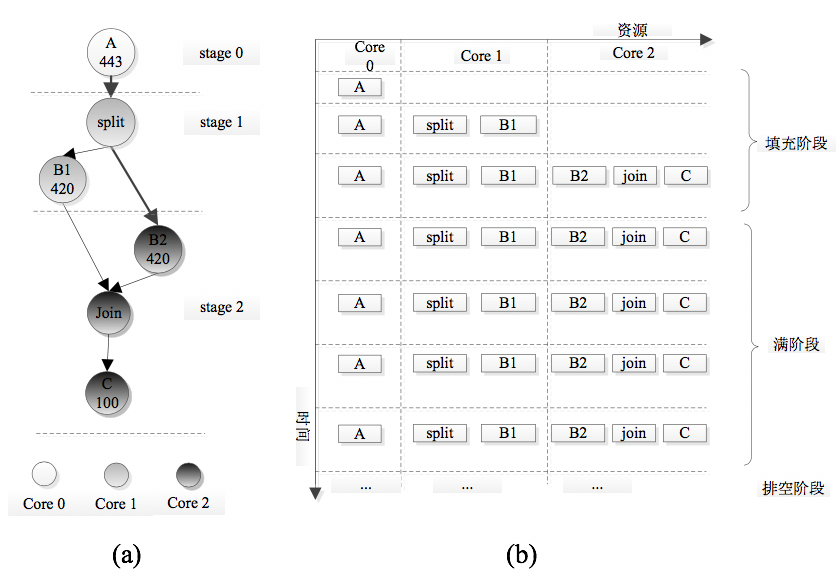
\includegraphics[width=0.8\textwidth]{Img/Chap_Application/Yu/streamline.png}\\
  \caption{(a)任务划分和阶段赋值的例子 (b)图(a)对应的软件流水执行过程}\label{fig:streamline}
\end{figure}

流水线执行过程分为三个阶段,分别是填充阶段、满阶段以及排空阶段。图\ref{fig:streamline}给出了任务划分、阶段赋值和软件流水调度执行的一个例子。初始SDF图 有A、B和C这3个计算节点,在任务划分阶段将B复制分裂成两个计算单元B1和B2,同时引入了split和join两个计算节点。经过任务划分后,计算单元A被分配到处理器核core0,split和B1被分配到core1,B2、join和C被分配到core2上。图\ref{fig:streamline}(a)给出了经过阶段赋值后各个计算单元的阶段值,完成了软件流水的构造。图\ref{fig:streamline}(b)给出了对应的软件流水调度执行过程,程序启动时流水线处于填充阶段,各个核上的计算节点按照其阶段值从小到大的顺序启动执行,当所有的计算节点都启动时,流水线进入满阶段;在流水线满阶段,所有的计算节点都进行周期性的迭代执行,由于任务划分阶段基本实现了不同计算核上的负载均衡,此时核间同步开销小,资源利用率高,系统的吞吐率达到最大;在流水线调度的排空阶段,程序开始相继结束计算节点的执行,各个核的计算节点按照阶段值从小到大的顺序结束其周期性的迭代,等到所有的计算节点结束其稳态调度后,整个程序终止并释放运行时占有的各种资源。

\subsubsection{性能评估}
为了对COStream编译系统面向X86架构的编译优化进行全面的性能评估和分析,选取了11个多媒体领域常见的算法作为测试程序用COStream数据流编程语言实现作为COStream编译器的输入。
\begin{figure}[htbp]
  \centering
  % Requires \usepackage{graphicx}
  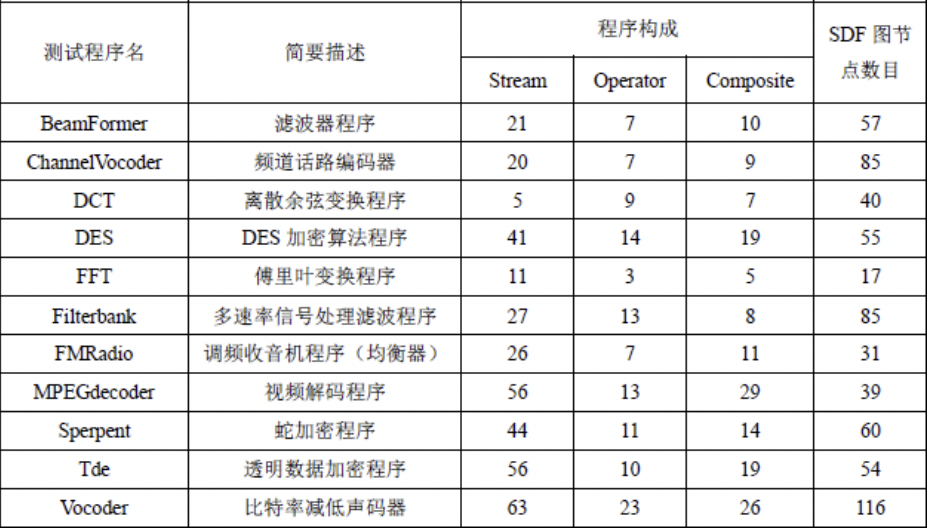
\includegraphics[width=0.8\textwidth]{Img/Chap_Application/Yu/x86benchmark.png}\\
  \caption{用于测试的数据流程序信息}\label{fig:x86benchmark}
\end{figure}

图\ref{fig:x86ratio}给出了测试程序经过COStream编译后在目标环境上执行的加速比。从图中可以看出,每个程序执行加速比随着处理核的数目增多而增加,基本呈现一个线性的加速情况。
\begin{figure}[htbp]
  \centering
  % Requires \usepackage{graphicx}
  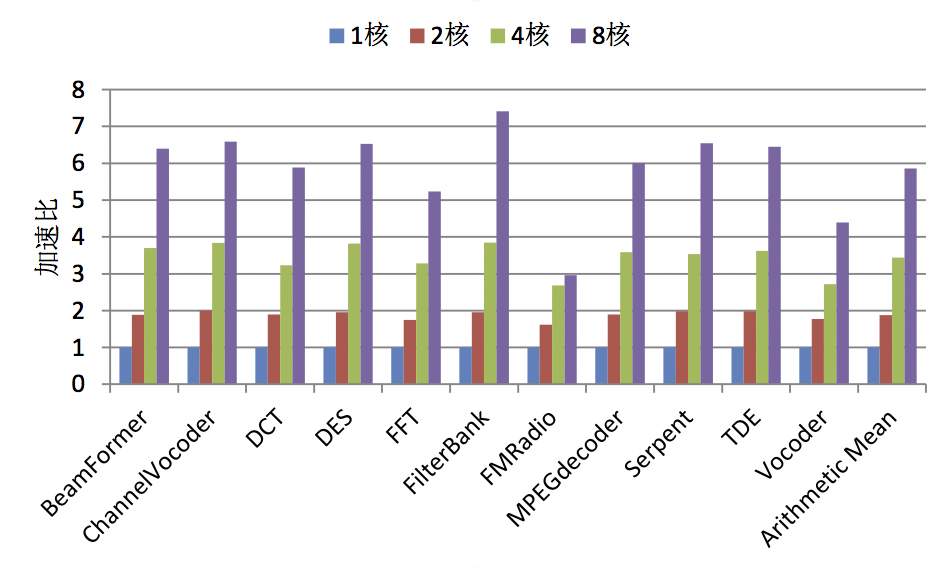
\includegraphics[width=0.8\textwidth]{Img/Chap_Application/Yu/x86ratio.png}\\
  \caption{测试代码在X86上达到的加速比}\label{fig:x86ratio}
\end{figure}

通信与同步比衡量了测试程序的有用计算和时间开销之间的比例,在一定程度上反应了程序的性能。在X86环境下采用的是软件流水调度策略,各个并行线程在软件流水调度的每次执行阶段中需要进行一次同步操作,COStream采用sense-reversing barrier[ ] 做核间的同步,保证不同核上的actor间的数据依赖关系能够满足。图\ref{fig:x86computeSync}给出了各个测试程序在8个核上的运行时计算同步时间分布。从图\ref{fig:x86computeSync}可以看出,FMRadio和Vocoder的计算同步比不太理想,同步开销太大,导致加速比较低,对于其他的测试程序计算同步比都能够达到较高水平,程序的加速比也较为理想。

\begin{figure}[htbp]
  \centering
  % Requires \usepackage{graphicx}
  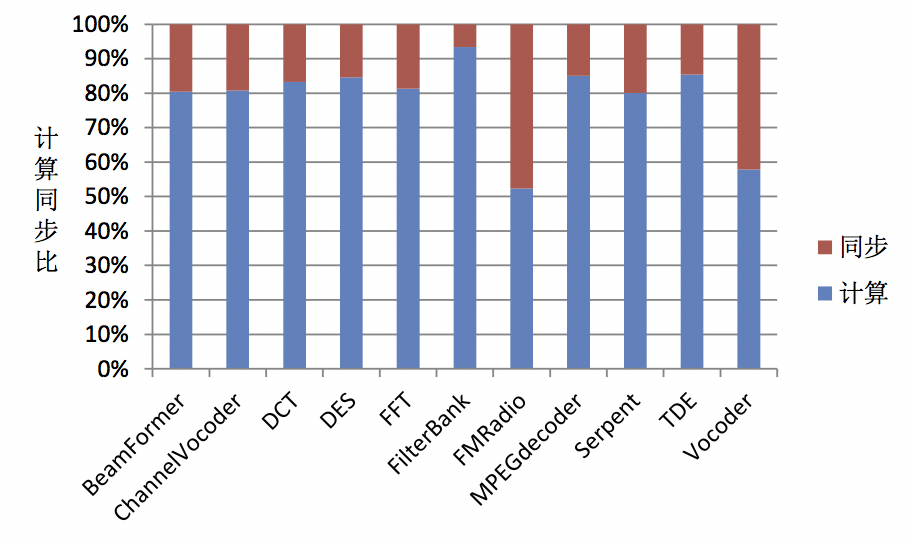
\includegraphics[width=0.8\textwidth]{Img/Chap_Application/Yu/x86computeSync.png}\\
  \caption{测试程序在8核上运行的计算同步比}\label{fig:x86computeSync}
\end{figure}




\subsection{相关工作}

\subsection{参考文献}
[1]魏海涛. 面向多核处理器的数据流程序编译关键技术研究(博士论文), 华中科技大学,2010.\\

[2] 张维维, 魏海涛, 于俊清, 李鹤, 黎昊, 杨秋吉. COStream:一种面向数据流的编程语言和编译器实现, 计算机学报, 2013, 36(10):1993 -2006

[3] Haitao Wei, Mingkang Qin, Junqing Yu, Dongrui Fan and Guang R. Gao. StreamTMC: Stream Compilation for Tiled Multi-core Architectures, Journal of Parallel and Distributed Computing (JPDC), 2013, 73(4): 484-494

[4] Haitao Wei, Junqing Yu, Huafei Yu, Mingkang Qin and Guang R. Gao. Software Pipelining for Stream Programs on Resource Constrained Multi-core Architecture, IEEE Transactions on Parallel and Distributed Systems, 2012, 23(12): 2338-2349

[5] Haitao Wei, Junqing Yu, Huafei Yu, Guangrong Gao. Minimizing Communication in Rate-Optimal Software Pipelining for Stream Programs, The 8th International Symposium on Code Generation and Optimization (CGO), 2010,Toronto, Canada, 210~217

[6] 魏海涛, 秦明康, 于俊清,范东睿. 一种面向众核架构的数据流编译框架, 计算机学报, 2014, 37(7): 1560-1569)

[7] 于俊清, 余华飞, 魏海涛, 秦明康. 多核环境下编译器辅助消息驱动的动态调度, 计算机学报, 2014, 37(7): 1633-1637

[8] 于俊清, 张维维, 陈文斌, 涂浩, 何云峰. 面向多核集群的数据流程序层次流水线并行优化方法研究, 计算机学报, 2014, 37(10): 2071-2083

[9] 魏海涛, 于俊清, 余华飞, 秦明康. 一种面向数据流程序的软件流水并行化方法, 计算机学报, 2011, 34(5): 889~898)

[10] 陈文斌,杨瑞瑞,于俊清. 基于GPU/CPU混合架构的流程序多粒度划分与调度方法研究, 计算机工程与科学,2017, 39(1): 15-26)

[11] 杨胜哲, 于俊清, 唐九飞. 数据流程序动态调度与优化方法研究, 计算机工程与科学,2017, 39(7): 1201-1210)

[12] 唐九飞, 李 鹤, 于俊清. 面向X86多核处理器的数据流程序任务调度与缓存优化, 中国科学技术大学学报, 2016, 46(3): 200-207

[13] 王兆吉. 利用COStream实现全连接和卷积神经网络的并行计算(硕士论文),2019,华中科技大学